\section{Oscillations}
\vocab{Free oscillation}: object oscillates with constant amplitude, with no external force acting on it

\begin{defn}{Amplitude $x_0$}{}
Magnitude of \underline{maximum displacement} from equilibrium position. 
\end{defn}

\begin{defn}{Period $T$}{}
Time taken for one complete oscillation. 
\end{defn}

\begin{defn}{Frequency $f$}{}
Number of complete cycles per unit time.
\end{defn}

\begin{defn}{Angular frequency $\omega$}{}
Measure of the rate of change of phase angle of the body's motion with time with respect to the centre of its oscillation.
\begin{equation} \omega = 2 \pi f = \frac{2\pi}{T}\end{equation}
\end{defn}
\pagebreak

\subsection{Kinematics}
\textbf{Displacement-time}:

When the body is at equilibrium position at $t=0$,
\begin{equation} x = x_0 \sin \omega t \end{equation}

\begin{figure}[H]
\centering
\begin{tikzpicture}
  \begin{axis}%
    [axis lines=middle,
     enlargelimits={abs=0.2},
     xlabel = $t$,
     ylabel = $x$,
     ticks=none
    ]
    \addplot[domain=0:12.57,samples=50,smooth,red] {sin(deg(x))};
  \end{axis}
\end{tikzpicture}
\end{figure}

When the body is at extreme position at $t=0$,
\[ x = x_0 \cos \omega t \]

\textbf{Velocity-time}:
\begin{equation} v = v_0 \cos \omega t \end{equation}

\begin{figure}[H]
\centering
\begin{tikzpicture}
  \begin{axis}%
    [axis lines=middle,
    enlargelimits={abs=0.2},
     xlabel = $t$,
     ylabel = $v$,
     ticks=none
    ]
    \addplot[domain=0:12.57,samples=50,smooth,red] {cos(deg(x))};
  \end{axis}
\end{tikzpicture}
\end{figure}
\pagebreak
\textbf{Acceleration-time}:
\begin{equation} a=-a_0\sin\omega t \end{equation}

\begin{figure}[H]
\centering
\begin{tikzpicture}
  \begin{axis}%
    [axis lines=middle,
    enlargelimits={abs=0.2},
     xlabel = $t$,
     ylabel = $a$,
     ticks=none
    ]
    \addplot[domain=0:12.57,samples=50,smooth,red] {-sin(deg(x))};
  \end{axis}
\end{tikzpicture}
\end{figure}

\textbf{Velocity-displacement}:
\begin{equation} v = \pm \omega \sqrt{{x_0}^2 - x^2} \end{equation}

\begin{figure}[H]
\centering
\begin{tikzpicture}
  \begin{axis}%
    [axis lines=middle,
    enlargelimits={abs=0.2},
     xlabel = $x$,
     ylabel = $v$,
     ticks=none,
     trig format plots=rad,variable=t
    ]    
    \addplot[domain=-2*pi:2*pi,samples=50,smooth,red]({10*cos(t)},{sin(t)});
  \end{axis}
\end{tikzpicture}
\end{figure}

\textbf{Acceleration-displacement}:\footnote{This is known as the defining equation of simple harmonic motion.}
\begin{equation} a = -\omega^2 x \end{equation}

\begin{figure}[H]
\centering
\begin{tikzpicture}
  \begin{axis}%
    [axis lines=middle,
    enlargelimits={abs=0.2},
     xlabel = $x$,
     ylabel = $a$,
     ticks=none
    ]    
    \addplot[domain=-6:6,samples=50,smooth,red] {-x};
  \end{axis}
\end{tikzpicture}
\end{figure}
\pagebreak

\begin{defn}{Phase}{}
Angle which gives a measure of the fraction of a cycle that has been completed by the oscillating particle or wave. 
\end{defn}

\begin{defn}{Phase difference $\phi$}{}
Angle which gives a measure of how much one oscillation is \underline{out of step} with another.
\end{defn}

\begin{itemize}
\item Graph of $x=x_0\cos(\omega t+\phi)$ is displaced to the left. Motion \textbf{leads} by time $\dfrac{\phi}{\omega}$.
\item Graph of $x=x_0\cos(\omega t-\phi)$ is displaced to the right. Motion \textbf{lags} by time $\dfrac{\phi}{\omega}$.
\end{itemize}

\begin{figure}[H]
\centering
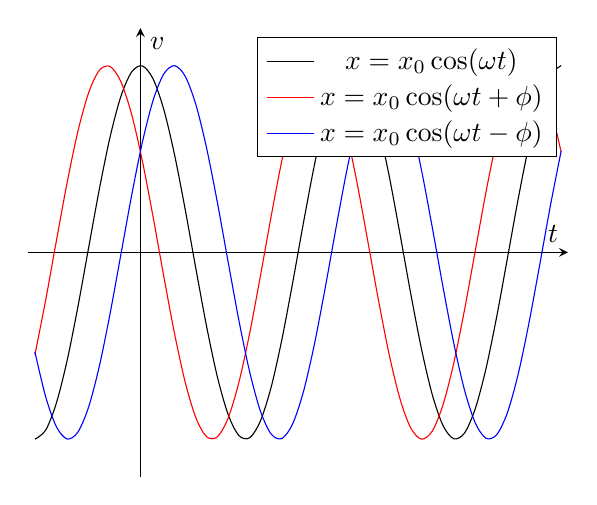
\begin{tikzpicture}
  \begin{axis}%
    [axis lines=middle,
    enlargelimits={abs=0.2},
     xlabel = $t$,
     ylabel = $v$,
     ticks=none
    ]
    \addplot[domain=-3.15:12.57,samples=50,smooth,black] {cos(deg(x))};
    \addlegendentry{$x=x_0\cos(\omega t)$}
    \addplot[domain=-3.15:12.57,samples=50,smooth,red] {cos(deg(x+1))};
    \addlegendentry{$x=x_0\cos(\omega t+\phi)$}
    \addplot[domain=-3.15:12.57,samples=50,smooth,blue] {cos(deg(x-1))};
    \addlegendentry{$x=x_0\cos(\omega t-\phi)$}
  \end{axis}
\end{tikzpicture}
\end{figure}
\pagebreak

\subsection{Energy}
For an oscillator in simple harmonic motion, total energy is sum of \textbf{kinetic energy} and \textbf{potential energy}.
\[ E=E_k+E_p \]
\begin{equation}
E_k = \frac{1}{2}m\omega^2{x_0}^2\cos^2 \omega t = \frac{1}{2}m\omega^2\brac{{x_0}^2-x^2}
\end{equation}
\begin{equation}
E_p = \frac{1}{2}m\omega^2{x_0}^2\sin^2 \omega t = \frac{1}{2}m\omega^2 x^2
\end{equation}
\[ E=E_{k,max}=E_{p,max}=\frac{1}{2}m\omega^2{x_0}^2 \]

Energy-time graph (for one period):
\begin{figure}[H]
\centering
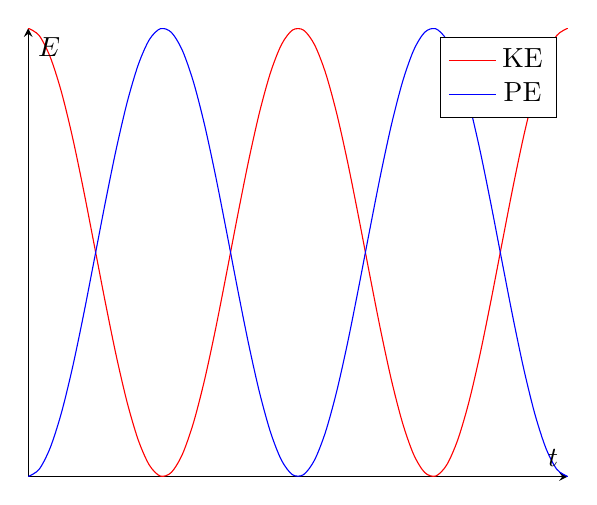
\begin{tikzpicture}
  \begin{axis}%
    [axis lines=middle,
     xlabel = \(t\),
     ylabel = {\(E\)},
     ticks=none
    ]
    \addplot[domain=0:12.57,samples=50,smooth,red] {cos(deg(x))+1};
    \addlegendentry{KE}
    \addplot[domain=0:12.57,samples=50,smooth,blue] {-cos(deg(x))+1};
    \addlegendentry{PE}
  \end{axis}
\end{tikzpicture}
\end{figure}

Energy-displacement graph (for one period):
\begin{figure}[H]
\centering
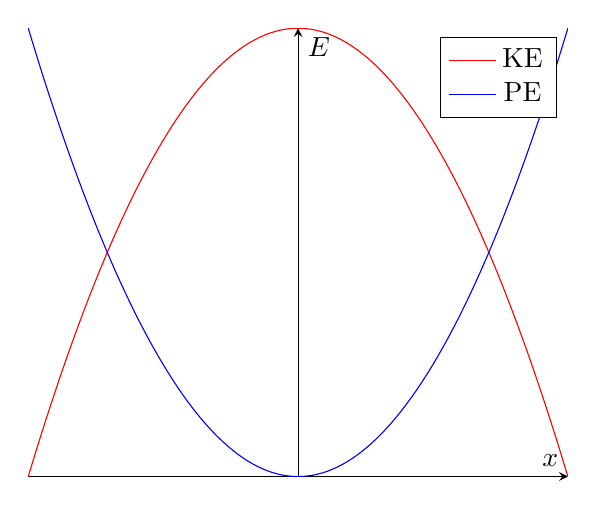
\begin{tikzpicture}
  \begin{axis}%
    [axis lines=middle,
     xlabel = \(x\),
     ylabel = {\(E\)},
     ticks=none
    ]
    \addplot[domain=-1:1,samples=50,smooth,red] {-x^2+1};
    \addlegendentry{KE}
    \addplot[domain=-1:1,samples=50,smooth,blue] {x^2};
    \addlegendentry{PE}
  \end{axis}
\end{tikzpicture}
\end{figure}
\pagebreak

\subsection{Simple harmonic motion}
\begin{defn}{Simple harmonic motion}{}
Oscillatory motion where acceleration is \underline{directly proportional} to displacement from a \underline{fixed point}, and this acceleration is always in the \underline{opposite direction} to its displacement.
\[ a \propto -x \]
\end{defn}

\subsubsection{Examples}
\textbf{Spring-mass system}

\begin{figure}[H]
    \centering
    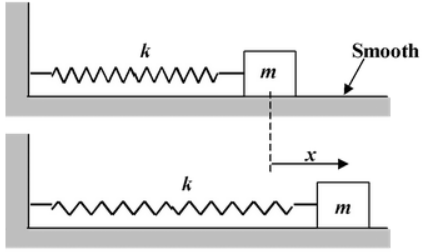
\includegraphics[width=8cm]{images/spring_mass_shm.png}
    \caption{Spring-mass system}
\end{figure}

Restoring force is $F=-kx$. By Newton's 2nd law, 
\[ \sum F=ma=-kx \implies a=-\frac{k}{m}x \]
Comparing with $a=-\omega^2x$,
\[ \omega = \sqrt{\frac{k}{m}} \]
Hence frequency is
\[ f=\frac{1}{2\pi}\sqrt{\frac{k}{m}} \]
\pagebreak

\textbf{Simple pendulum}

\begin{figure}[H]
    \centering
    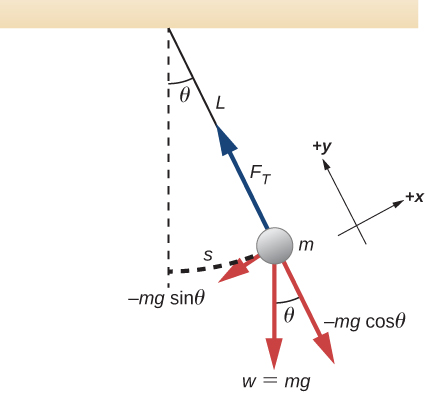
\includegraphics[width=8cm]{images/simple_pendulum_shm.jpg}
    \caption{Simple pendulum}
\end{figure}

Restoring force is the component of the bob's weight, $mg\sin\theta$, that is tangential to the circumference of its swing. 

For small $\theta$, by small angle approximation, $mg\sin\theta \approx mg\theta$, where $\theta\approx\frac{x}{l}$.

By Newton's 2nd Law, 
\[ \sum F=ma=-mg\theta=-\frac{mgx}{l} \implies a=-\frac{g}{l}x \]

Comparing with $a=-\omega^2x$,
\[ \omega=\sqrt{\frac{g}{l}} \]

Hence frequency is
\[ f=\frac{1}{2\pi}\sqrt{\frac{g}{l}} \]
This indicates that the angular velocity or the period of a simple pendulum is independent of the mass of the weight and the amplitude of oscillation. This is called Galileo's \textbf{isochronism of pendulum}.
\pagebreak

\textbf{Vertical spring-mass system}

\begin{figure}[H]
    \centering
    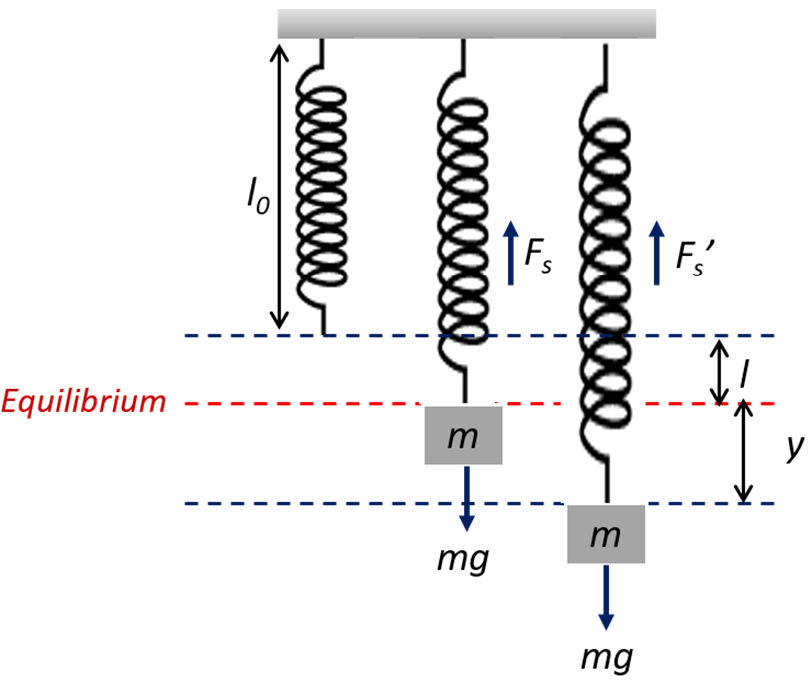
\includegraphics[width=8cm]{images/vertical_spring_mass_shm.png}
    \caption{Vertical spring-mass system}
\end{figure}

At equilibrium, spring force balances weight: $ke=mg$.

At lowest point, by Newton's 2nd law,
\[ \sum F=mg-k(e+x)=ma \implies a=-\frac{k}{m}x \]

Comparing with $a=-\omega^2x$,
\[ \omega^2=\frac{k}{m} \implies f=\frac{1}{2\pi}\sqrt{\frac{k}{m}} \]
\pagebreak

\textbf{Floating block}

\begin{figure}[H]
    \centering
    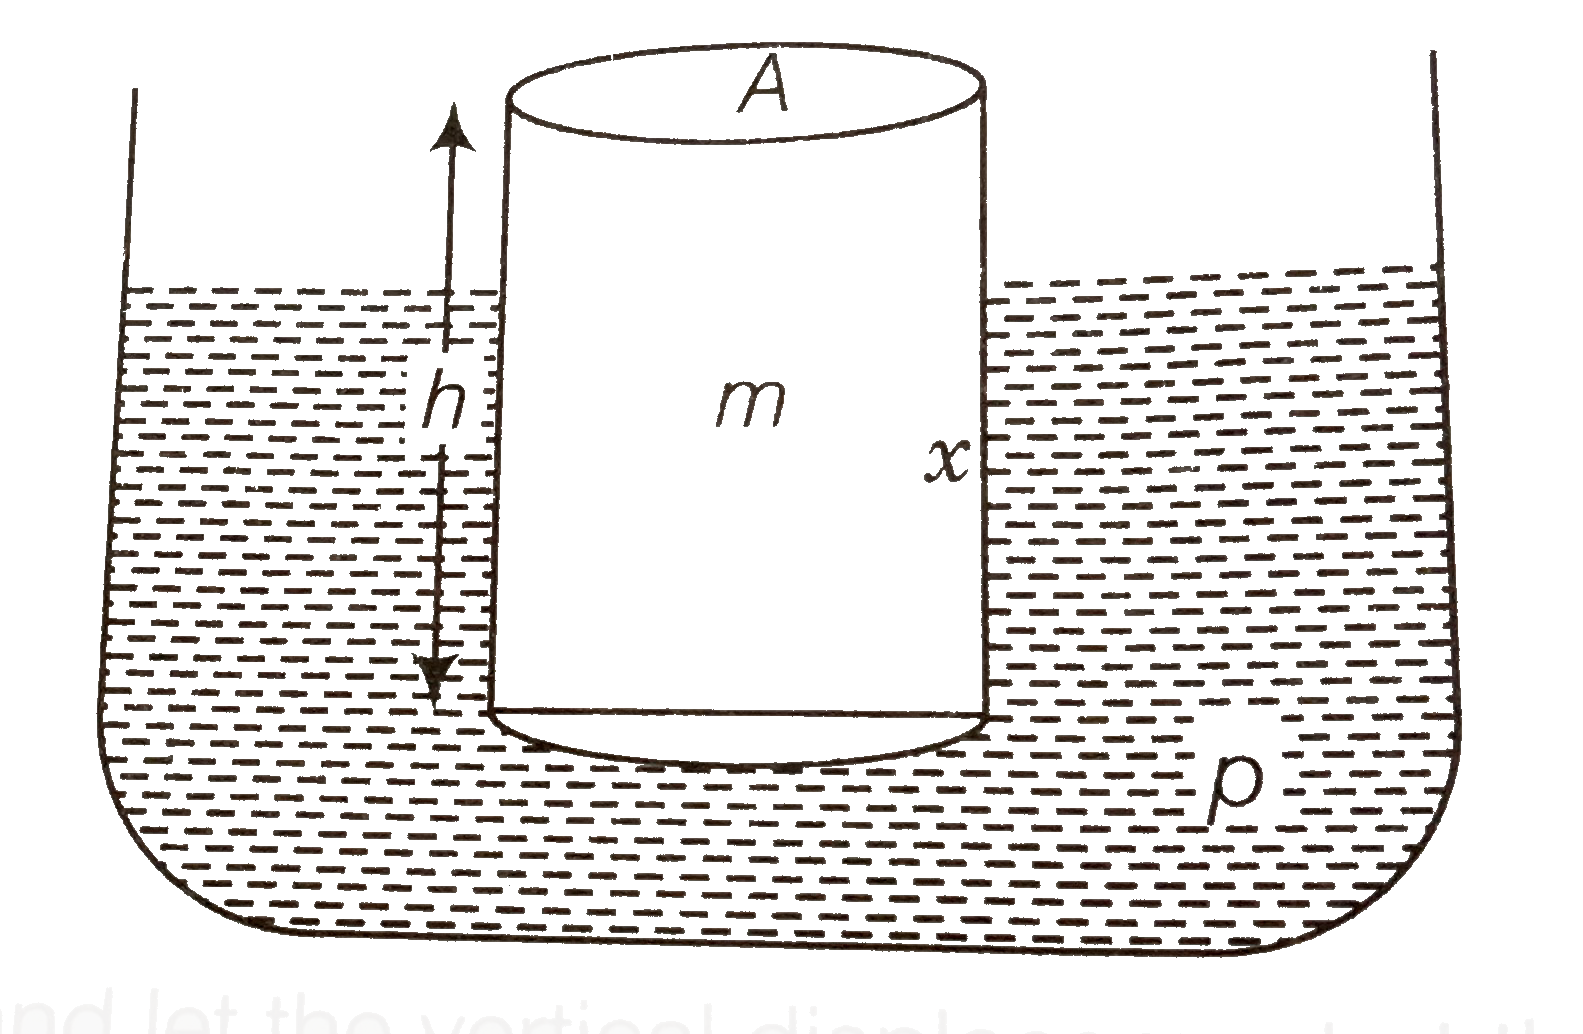
\includegraphics[width=8cm]{images/floating_block_shm.png}
    \caption{Floating block}
\end{figure}

Restoring force is the difference between upthrust exerted by water on block and the block's weight. By Newton's 2nd law,
\[ \sum F=mg-\rho(A(h+x))g = -\rho(Ax)g = ma \implies a=-\frac{\rho Ag}{m}x \]

Comparing with $a=-\omega^2x$,
\[ \omega=\sqrt{\frac{\rho Ag}{m}} \]
Hence frequency is 
\[ f=\frac{1}{2\pi}\sqrt{\frac{\rho Ag}{m}} \]
\pagebreak


\subsection{Damped oscillation}
\begin{defn}{Damping}{}
\underline{Energy is lost} from system as a result of \underline{dissipative forces.}
\end{defn}

\begin{defn}{Damped oscillation}{}
\underline{Amplitude decreases with time} due to loss of energy to surroundings as a result of resistive forces acting on system.
\end{defn}

Degrees of damping:
\begin{enumerate}
\item \textbf{Light damping}: continues to oscillate, amplitude decreases gradually with time but period remains almost the same
\item \textbf{Heavy damping}: does not oscillate, takes a long time to return to equilibrium\\ e.g. door damper
\item \textbf{Critical damping}: does not oscillate, returns to equilibrium in the shortest possible time\\ e.g. damping system of car
\end{enumerate}

\begin{figure}[H]
    \centering
    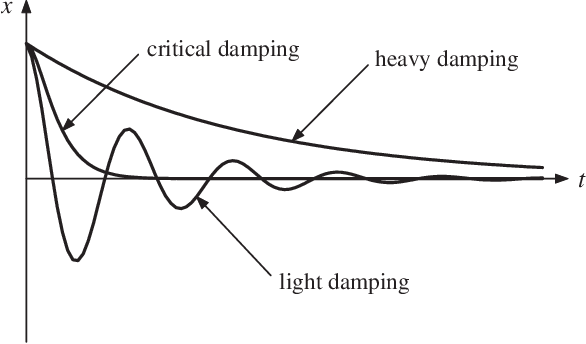
\includegraphics[width=11cm]{images/Damping.png}
\end{figure}

The equation for undamped free oscillation is 
\[ x=x_0\cos\omega t \]
The equation for damped oscillation is 
\[ x=x_0e^{-\frac{b}{2m}t}\cos\omega t \]
where $b$ is the damping constant.
\pagebreak

\subsection{Forced oscillation}
\begin{defn}{Forced oscillation}{}
Continual \underline{input of energy} by an external applied force, to compensate the energy loss due to damping, in order to maintain amplitude of oscillation.

The system oscillates at the frequency of the external periodic force.
\end{defn}

\subsection{Resonance}
\begin{defn}{Natural frequency $f_0$}{}
Frequency at which a body oscillates after an initial disturbance. 
\end{defn}

\begin{defn}{Resonance}{}
Amplitude of the oscillator reaches a maximum when driving frequency equals natural frequency of the oscillator, resulting in maximum transference of energy to the oscillator.
\[ f=f_0 \]
\end{defn}

Amplitude of forced oscillation changes with driving frequency. When $f=f_0$, \underline{resonance} occurs, amplitude is maximum.

\begin{figure}[H]
    \centering
    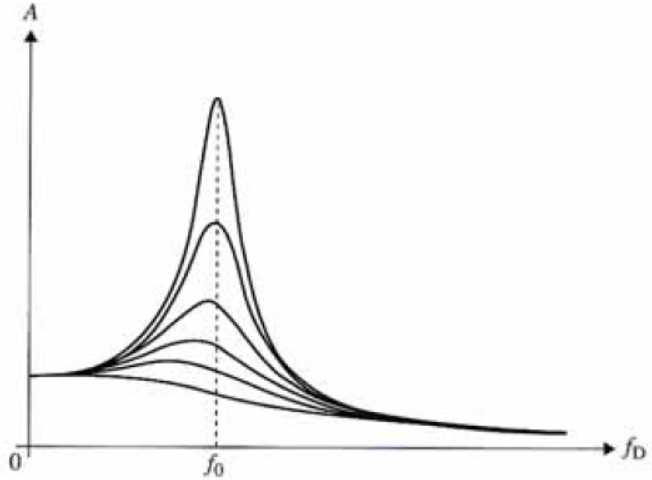
\includegraphics[width=10cm]{images/Amptlitude_forced_oscillation.png}
\end{figure}

Effect of increased damping on resonance curve:
\begin{itemize}
\item Lower at all frequencies
\item Flatter peak
\item Peak shifts to left slightly
\end{itemize}

\textbf{Applications of resonance:} magnetic resonance imaging (MRI)

\textbf{Drawbacks of resonance:} bridge design to prevent collapse due to resonant oscillations
\pagebreak

\subsection*{Problems}
\begin{prbm}
A cylinder of radius $R$, length $h$, density $\rho_0$ floats upright in a fluid of density $\rho_1$. It is given a small vertical displacement, and undergoes undamped harmonic motion with angular frequency $\omega$. 

Calculate $\omega^2$.
\end{prbm}

\begin{proof}[Solution]
Using Archimedes’ principle: the force on the cylinder is equal to the weight of the water displaced, which is
\[ F = mg = -\rho_1 (\pi R^2 d)g \]
where $d$ is the vertical displacement. 

This acts as a spring force $F=-kd$. The spring constant $k$ of a harmonic oscillator of mass $m$ is related to the angular frequency $\omega$ by $k=m\omega^2$; in this case, mass $m=\rho_0 \cdot \pi R^2h$.

Putting everything together, 
\[ k=\rho_1\pi R^2 g = \rho_0\pi R^2 h\omega^2 \]
\[ \boxed{\omega^2=\frac{\rho_1g}{\rho_0h}} \]
\end{proof}
\pagebreak

\begin{prbm}
The figure below shows a simple pendulum consisting of a small mass at the end of a light, inextensible string. It swings from an initial position of $\theta=10\degree$, for which it would have a period $T_0$. It hits a slanted wall elastically, which is at angle $\phi=5\degree$ to the vertical.

\begin{figure}[H]
    \centering
    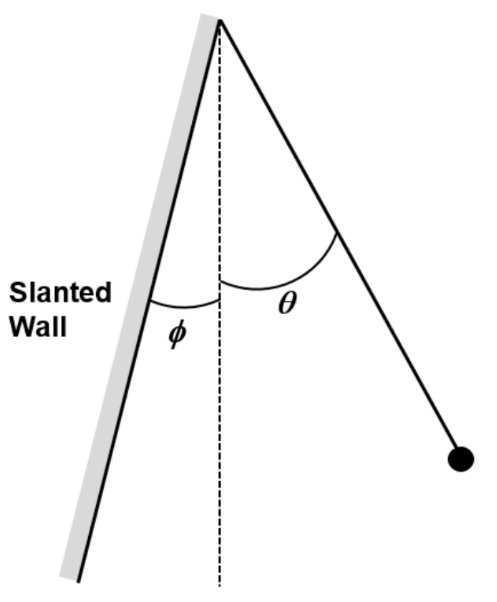
\includegraphics[width=6cm]{images/pendulum_wall.png}
\end{figure}

When the pendulum hits the wall, what is the new period of oscillation, in terms of $T_0$?
\end{prbm}

\begin{proof}[Solution]
Simple harmonic motion implies $\theta = \theta_0 \cos \omega t$, where $\theta_0 = 10\degree$ before the collision, and given the period we know $\omega = \dfrac{2\pi}{T_0}$.

Let $T$ be time taken to swing from initial position to $-5\degree$.
\[ -5\degree = 10\degree \cos \frac{2\pi T}{T_0} \implies \frac{2\pi T}{T_0} = \frac{2\pi}{3} \implies T=\frac{T_0}{3} \]

Hence new period is $\boxed{\dfrac{2T_0}{3}}$.
\end{proof}

\pagebreak